\documentclass[11pt,letter]{article}
\usepackage[top=1.00in, bottom=1.0in, left=1.1in, right=1.1in]{geometry}
\renewcommand{\baselinestretch}{1.6}
\usepackage{graphicx}
\usepackage{natbib}
\usepackage{amsmath}
\usepackage{amssymb} 
\usepackage{lineno}
\usepackage{xr-hyper}
\externaldocument{decsens_supp}
\newcommand{\R}[1]{\label{#1}\linelabel{#1}}
\usepackage{hyperref}

\def\labelitemi{--}
\parindent=0pt
\begin{document}

\title{A simple explanation for declining temperature sensitivity \\ with warming} % The illusion of declining temperature sensitivity with warming // Sensitivities are not declining with warming OR As climate change accelerates biology, chasing statistical artifacts ensues
\author{E. M. Wolkovich$^{1,a}$,  J. L. Auerbach$^{2}$, \\C. J. Chamberlain (ORCID: 0000-0001-5495-3219)$^{3}$, D. M. Buonaiuto (0000-0003-4022-2591)$^{3}$, \\ A. K. Ettinger (0000-0002-6228-6732)$^4$, I. Morales-Castilla$^{5}$ \& A. Gelman$^{2}$} 
\date{} %\today
\maketitle
$^1$Forest \& Conservation Sciences, Faculty of Forestry, University of British Columbia, Vancouver, British Columbia, Canada\\
$^2$Department of Statistics, Columbia University, New York, NY 10027, USA\\
$^3$Department of Organismic and Evolutionary Biology, Harvard University, Cambridge, Massachusetts, USA\\
$^4$The Nature Conservancy in Washington, 74 Wall Street, Seattle, WA, USA\\
$^5$University of Alcal\`a, Global Change Ecology and Evolution Group-GloCEE, Department of Life Sciences, CTRA N-II, KM., 33,600, 28802, Madrid, Spain\\
$^a$Corresponding author (ORCID: 0000-0001-7653-893X); e.wolkovich@ubc.ca; 604.827.5246
\vspace{3ex}

\emph{Running title:} Declining temperature sensitivity\\
\emph{Article type}: Perspective\\

\newpage
\begin{abstract} % 132 words
Recently, multiple studies have reported declining phenological sensitivities ($\Delta$ days per $^{\circ}$C) with higher temperatures. Such observations have been used to suggest climate change is reshaping biological processes, with major implications for forecasts of future change. Here we show that these results may simply be the outcome of using linear models to estimate non-linear temperature responses, specifically for events that occur after a cumulative thermal threshold is met---a common model for many biological events. Corrections for the non-linearity of temperature responses consistently remove the apparent decline. Our results show that rising temperatures combined with linear estimates based on calendar time produce observations of declining sensitivity---without any shift in the underlying biology. Current methods may thus undermine efforts to identify when and how warming will reshape biological processes.
\end{abstract}
\vspace{5ex}


\newpage
% \linenumbers
\section{Main text} % 1103 right now; ack: 66; datacode: 44; author contr: 41
Climate change has reshaped biological processes around the globe, with shifts in the timing of major life history events (phenology), carbon dynamics and other ecosystem processes. With rising temperatures,  a growing body of literature has documented changes in temperature sensitivity---the magnitude of a biological response scaled per $^{\circ}$C. Many studies have found declining responses to temperature in recent decades \citep{fu2015,piao2017} or lower sensitivities in warmer, urban areas \citep{meng2020}.\\

Most studies attribute changes in temperature sensitivity to shifts in underlying biological processes. Researchers have suggested weaker temperature sensitivities are evidence of increased light limitation in the tundra \citep{piao2017}, or a decline in the relative importance of warm spring temperatures for spring phenological events (e.g., leafout, insect emergence) in the temperate zone \citep{fu2015,meng2020}, as other environmental triggers (e.g., winter temperatures that determine `chilling') play a larger role. Yet, despite an increase in studies reporting declining or shifting temperature sensitivities, none have provided strong evidence of the biological mechanisms underlying these changes  \citep[e.g.,][]{fu2015,meng2020}. The missing mechanisms may be hidden in the data: environmental factors moderate biological processes in complex ways \citep{chuine2016}, are strongly correlated in nature \citep[e.g.,][]{fu2015}, and temperature variance shifts over time and space \citep{keenan2019}. \\


Here we propose a simpler alternative explanation: the use of linear models for non-linear responses to temperature. Researchers generally use methods with assumptions of linearity to calculate temperature sensitivities, often relying on some form of linear regression to compute a change in a quantity---days to leafout or carbon sequestered over a fixed time, for example---per $^{\circ}$C, thus ignoring that many biological responses to temperature, especially events, are non-linear (Fig. \ref{fig:ospreewsims}). \\ 

Many observed biological responses are the result of continuous non-linear processes that depend on temperature, which are discretized into temporal units for measurement. For example, a biological response, such as leafout, occurs when a certain thermal sum is reached, and plants will reach this threshold more quickly---in calendar time---when average daily temperatures are warmer \citep[Fig. \ref{fig:ospreewsims},][]{kramer2012book}. 
Biologically, however, the plants require the same temperature sum to trigger leafout at high and low average temperatures. Indeed any process observed or measured as the time until reaching a threshold is inversely proportional to the speed at which that threshold is approached. \\ 

Temperature determines the speed of many biological processes. Thus, at very low temperatures plants would never leaf out and at higher temperatures they could leaf out in only a matter of days---yet sensitivities estimated from linear regression at higher (warmer) temperatures would appear much lower than those observed at lower temperatures. Using a simple model where leafout occurs after a thermal sum is met we can hold the temperature threshold for leafout constant \citep{zohner2020gcb} and examine how estimated sensitivities (measured in days per $^{\circ}$C using linear regression) shift with warming. In this simple thermal sum model \citep[which we argue is the null model for studies of biological events across different temperatures, Fig. \ref{fig:ospreewsims} and][]{kramer2012book,zohner2020gcb} we find declining sensitivities with warming (Fig \ref{fig:basicsims}; see `A first-hitting-time model of leafout' in Supporting Information for a full derivation of the statistical properties). Indeed, under this model constant temperature sensitivity would be evidence that the temperature threshold is not constant and the mechanisms underlying the leafout process have changed. \\


Correcting for non-linearity using the transformation for an inverse relationship (log transformation) removes apparent declines in temperature sensitivity in long-term leafout and harvest data (Fig. \ref{fig:basicsimswpep}-\ref{fig:wine}, \ref{fig:basicsims}, \href{https://github.com/temporalecologylab/labgit/tree/master/projects/decsenspost}{code link}). In empirical long-term tree leafout data from Europe, correcting for non-linearity in responses produces little evidence for declining sensitivities with warming (Figs. \ref{fig:basicsimswpep}). An apparent decline in sensitivity for silver birch (\emph{Betula pendula}) from -4.3 days/$^{\circ}$C to -3.6 days/$^{\circ}$C from 1950-1960 compared to 2000-2010 disappears using a log-log regression (-0.17 versus -0.22). Moreover, the variance of the leafout dates declines as temperatures rise---(declines of roughly 50\%, see Tables \ref{tab:pep10yr}-\ref{tab:pep20yr}), which is expected under our model as warming accelerates towards the thermal threshold that triggers leafout \citep[and in contrast to predictions from changing mechanisms, see][]{ford2016}. A similar apparent decline in winegrape harvest data in Burgundy disappears with a log transformation (estimates of -7.1 days/$^{\circ}$C to -6.5 days/$^{\circ}$C from 1951-1979 compared to 1980-2007 are both estimated as -1.4 using log-log regression), and an increase in sensitivity in Bordeaux, which has warmed substantially, becomes larger in relative magnitude (-6.8 days/$^{\circ}$C from 1951-1979 compared to -7.2 from 1980-2007 become -1.4 and -1.7, respectively, using log-log regression). \\
% PEP725 #s are in supp ... 
% for wine: check out plotburdat and plotborddat in decsenswine.R 
% We see similar corrections using 20-year windows, and a potential increase in sensitivity for European beech (\emph{Fagus sylvatica}, see Tables \ref{tab:pep10yr}-\ref{tab:pep20yr}). 

Fundamentally rising temperatures should alter many biological processes, making robust methods for identifying these changes critical. In spring plant phenology, where declining sensitivities are often reported \citep{fu2015,piao2017}, warming may increase the role of `chilling' (determined mainly by winter temperatures) and daylength---potentially increasing the thermal sum required for leafout at lower values of these cues \citep{Laube:2014a}. Adjusting our simulations to match this model yielded shifts in sensitivities with warming. After correcting for non-linearity, the shifts in sensitivities remained and they occurred in step with the biological change (Fig. \ref{fig:simsshiftcues}a, c). In contrast, sensitivities estimated from a linear model showed shifts across the entire range of warming, well before the simulated biological change (Fig. \ref{fig:simsshiftcues}a, c). Further, we found that an increase in the thermal sum required for leafout should yield larger in magnitude temperature sensitivities, not smaller, as is often expected \citep[e.g.,][]{fu2015}. \\ 

\emph{Conclusion}\\
Our results highlight the complexity of identifying what trends to expect in sensitivities with warming, and suggest that without useful null models we may misinterpret when biological change occurs. Inferring biological processes from statistical artifacts is not a new problem \citep[e.g.,][]{nee2005}, but climate change provides a new challenge in discerning mechanism from measurements because it affects biological time, while researchers continue to use calendar time. Other fields focused on temperature sensitivity often use approaches that acknowledge the non-linearity of responses (e.g., $Q_{10}$). Researchers have called for greater use of process-based models \citep{keenan2019}, which often include non-linear responses to temperature, but process-based models themselves rely on exploratory methods and descriptive analyses for progress \citep{chuine2016}. The challenge, then, is to interrogate the implicit and explicit models we use to interpret data summaries, and to develop null expectations that apply across biological and calendar time. \\


\begin{thebibliography}{10}
\providecommand{\natexlab}[1]{#1}

\bibitem[{Chuine et~al.(2016)Chuine, Bonhomme, Legave, Garc{\'\i}a~de
  Cort{\'a}zar-Atauri, Charrier, Lacointe, and Am{\'e}glio}]{chuine2016}
Chuine, I., M.~Bonhomme, J.-M. Legave, I.~Garc{\'\i}a~de Cort{\'a}zar-Atauri,
  G.~Charrier, A.~Lacointe, and T.~Am{\'e}glio. 2016.
\newblock Can phenological models predict tree phenology accurately in the
  future? {T}he unrevealed hurdle of endodormancy break.
\newblock Global Change Biology 22:3444--3460.

\bibitem[{Ford et~al.(2016)Ford, Harrington, Bansal, Gould, and
  St.~Clair}]{ford2016}
Ford, K.~R., C.~A. Harrington, S.~Bansal, J.~Gould, Peter, and J.~B. St.~Clair.
  2016.
\newblock Will changes in phenology track climate change? {A} study of growth
  initiation timing in coast {Douglas--fir}.
\newblock Global Change Biology 22:3712--3723.

\bibitem[{Fu et~al.(2015)Fu, Zhao, Piao, Peaucelle, Peng, Zhou, Ciais, Huang,
  Menzel, Uelas, Song, Vitasse, Zeng, and Janssens}]{fu2015}
Fu, Y. S.~H., H.~F. Zhao, S.~L. Piao, M.~Peaucelle, S.~S. Peng, G.~Y. Zhou,
  P.~Ciais, M.~T. Huang, A.~Menzel, J.~P. Uelas, Y.~Song, Y.~Vitasse, Z.~Z.
  Zeng, and I.~A. Janssens. 2015.
\newblock Declining global warming effects on the phenology of spring leaf
  unfolding.
\newblock Nature 526:104--107.

\bibitem[{Keenan et~al.(2020)Keenan, Richardson, and Hufkens}]{keenan2019}
Keenan, T.~F., A.~D. Richardson, and K.~Hufkens. 2020.
\newblock On quantifying the apparent temperature sensitivity of plant
  phenology.
\newblock New Phytologist 225:1033--1040.

\bibitem[{Kramer(2012)}]{kramer2012book}
Kramer, P. 2012.
\newblock Physiology of woody plants.
\newblock Elsevier, New York.

\bibitem[{Laube et~al.(2014)Laube, Sparks, Estrella, H{\"o}fler, Ankerst, and
  Menzel}]{Laube:2014a}
Laube, J., T.~H. Sparks, N.~Estrella, J.~H{\"o}fler, D.~P. Ankerst, and
  A.~Menzel. 2014.
\newblock Chilling outweighs photoperiod in preventing precocious spring
  development.
\newblock Global Change Biology 20:170--182.

\bibitem[{Meng et~al.(2020)Meng, Mao, Zhou, Richardson, Lee, Thornton,
  Ricciuto, Li, Dai, Shi, and Jia}]{meng2020}
Meng, L., J.~Mao, Y.~Zhou, A.~D. Richardson, X.~Lee, P.~E. Thornton, D.~M.
  Ricciuto, X.~Li, Y.~Dai, X.~Shi, and G.~Jia. 2020.
\newblock {Urban warming advances spring phenology but reduces the response of
  phenology to temperature in the conterminous United States}.
\newblock Proceedings of the National Academy of Sciences 117:4228.

\bibitem[{Nee et~al.(2005)Nee, Colegrave, West, and Grafen}]{nee2005}
Nee, S., N.~Colegrave, S.~A. West, and A.~Grafen. 2005.
\newblock The illusion of invariant quantities in life histories.
\newblock Science 309:1236--1239.

\bibitem[{Piao et~al.(2017)Piao, Liu, Wang, Peng, Ciais, Huang, Ahlstrom,
  Burkhart, Chevallier, Janssens et~al.}]{piao2017}
Piao, S., Z.~Liu, T.~Wang, S.~Peng, P.~Ciais, M.~Huang, A.~Ahlstrom, J.~F.
  Burkhart, F.~Chevallier, I.~A. Janssens, et~al. 2017.
\newblock Weakening temperature control on the interannual variations of spring
  carbon uptake across northern lands.
\newblock Nature Climate Change 7:359.

\bibitem[{Zohner et~al.(2020)Zohner, Mo, Pugh, Bastin, and
  Crowther}]{zohner2020gcb}
Zohner, C.~M., L.~D. Mo, T.~A.~M. Pugh, J.~F. Bastin, and T.~W. Crowther. 2020.
\newblock Interactive climate factors restrict future increases in spring
  productivity of temperate and boreal trees.
\newblock Global Change Biology 26:4042--4055.

\end{thebibliography}

\vspace{5ex}

\emph{Acknowledgements:} Thanks to TJ Davies, TM Giants, Y. Fu, D. Lipson, C. Rollinson, Y. Vitasse, and anonymous reviewers for comments that improved the manuscript.  NSERC (grant RGPIN­05038 to EMW), Canada Research Chair in Temporal Ecology (EMW), the Spanish Ministry for Science and Innovation (grant PID2019/109711RJ-I00 to IM-C) and Comunidad de Madrid and Universidad de Alcal\'a (grant CM/BG/2021-003 to IM-C) provided funding. 
\\ % and C. Zohner.

\emph{Data \& Code Availability:} Code for simulations, empirical analysis, and plots is provided \href{https://github.com/temporalecologylab/labgit/tree/master/projects/decsenspost}{here}. For empirical examples, data are available through \href{https://knb.ecoinformatics.org}{the OSPREE database}, \href{http://www.pep725.eu/data.php}{PEP 725 phenological data}, \href{https://surfobs.climate.copernicus.eu/dataaccess/access_eobs.php}{E-OBS climate data} and \href{https://www.ncdc.noaa.gov/data-access/paleoclimatology-data/datasets}{NOAA Paleoclimate Archive}. All data are freely available via the links.\\

\emph{Author contributions:} All authors contributed to idea development and editing the manuscript. In addition, EMW wrote the manuscript, developed the simulations, and made the figures; JLA formalized the first-hitting time model and its derivations, CJC did much of the PEP725 analysis.\\

\emph{List of Supporting Information:}\\
A first-hitting-time model of leafout\\
Simulations of common hypotheses for declining sensitivity\\
Additional methods \& results from long-term empirical data\\
Table S1-S2\\
Fig S1-S6

\newpage
\section* {Figures}

\begin{figure}[h!]
\centering
% \noindent 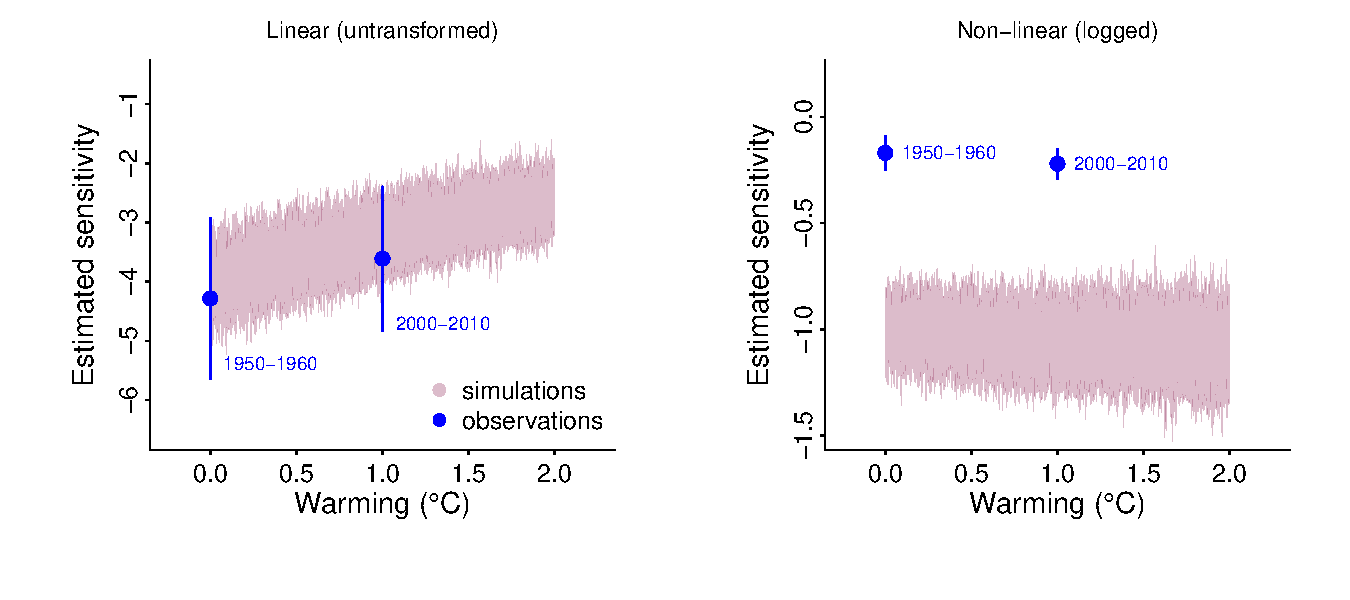
\includegraphics[width=1.05\textwidth]{..//analyses/figures/basicsimsandpepalt1.pdf} % 136 words
\caption{\textbf{Shifts in temperature sensitivities (response per $^{\circ}$C) with warming occur when using linear models for non-linear processes.} Estimated sensitivities decline (in magnitude) with warming in simulations (shading) with no underlying change in the biological process when sensitivities were estimated with linear regression (left; we simulated leafout for 45 sites as occurring after a certain thermal sum is met, simulating spring temperatures using draws from a normal(6,4), variation comes from fluctuation in the Monte Carlo simulations). This decline disappears when performing the regression on logged predictor and response variables (right). Such issues may underlie declining sensitivities calculated from observational data, including long-term observations of leafout across Europe (for \emph{Betula pendula} from PEP725 from for the 45 sites that had complete data for 1950-1960 and 2000-2010), which show a lower sensitivity with warming when calculated on raw data, but no change in sensitivity using logged data. Shading, symbols and lines represent means $\pm$ standard deviations of regressions across sites. See Supporting Information for a discussion of why estimated sensitivities are -1 in simulations in non-linear models.} 
\label{fig:basicsimswpep} % decsensSims.R
\end{figure}


\end{document}

